\chapter{RESULTADOS E DISCUSSÕES}
\label{cha:resultados}

% Cabeçalho de tabela em mais de uma linha, centrado verticalmente e sem invadir a borda.
\providecommand{\cabecalho}[1]{\begin{tabular}[c]{@{}c@{}}#1\end{tabular}}

Este capítulo apresenta os resultados das duas verificações propostas no Capítulo~1: se a planta simulada se comporta como o modelo de Downs e Vogel e se o veredito do Kubernetes acompanha a planta, em operação normal e sob distúrbio, com a política fixa. Os dados vêm das gravações feitas no laboratório da Seção~\ref{subsec:lab_kind} e do registro de experimentos do projeto. Nenhuma rodada foi repetida para este texto.

% -------------------------------------------------------------------------
\section{Como os experimentos foram feitos}
\label{sec:metodo_exp}

Todas as rodadas usaram o laboratório descrito na Seção~\ref{sec:supervisor}, com o supervisor no \textit{cluster} Kind, avaliando a política do Modo~1 (Seção~\ref{subsec:politica_modo1}). A planta, o \textit{historian} e a IHM rodaram direto no VS Code, sem o Docker Compose, o que não muda a forma como eles conversam (Seção~\ref{sec:arquitetura}). A planta rodou com ruído nos sensores. A velocidade da simulação e os distúrbios foram comandados pelo UaExpert, e cada rodada foi gravada pelos \textit{scripts} \texttt{record\_run.py}, com o veredito do supervisor, e \texttt{record\_signals.py}, com os sinais que o \textit{status} não traz. O supervisor avalia a planta a cada 30~s de relógio, e as contagens deste capítulo são feitas por avaliação.

As rodadas usaram duas velocidades: 5, em que a planta anda cerca de 10 vezes mais rápido que o tempo real, e 30, em que anda cerca de 56 vezes mais rápido. A resposta da planta não depende da velocidade, porque a física avança sempre 1~s de processo por passo. O que muda é o que o supervisor enxerga, porque as janelas dele são medidas em tempo de relógio (Seção~\ref{subsec:series}). À velocidade 5, cada avaliação cobre cerca de 5 minutos de processo; à velocidade 30, cerca de 28 minutos, e a janela de 300~s do índice das malhas cobre cerca de 4,7~h. Por isso, os tempos de veredito e os índices das rodadas à velocidade 30 não se comparam diretamente com os das rodadas à velocidade 5. A Tabela~\ref{tab:rodadas} resume as rodadas.

\begin{table}[htbp]
	\centering
	\caption{Rodadas usadas neste capítulo.}
	\label{tab:rodadas}
	\scriptsize
	\begin{tabular}{|>{\raggedright\arraybackslash}p{0.15\textwidth}|c|>{\raggedright\arraybackslash}p{0.14\textwidth}|c|c|c|c|>{\raggedright\arraybackslash}p{0.12\textwidth}|}
		\hline
		\textbf{Rodada} & \textbf{Data} & \textbf{Versão} & \textbf{Malhas} & \textbf{Veloc.} & \cabecalho{\textbf{Tempo}\\\textbf{simulado (h)}} & \textbf{Aval.} & \textbf{Distúrbio} \\
		\hline
		Calibração & 08/10 & 2.0.0 & P & 5 & 1,75 a 5,06 & 41 & nenhum \\
		Experimento 25 & 08/10 & 2.0.0 & P & 5 & 1,39 a 4,93 & 44 & IDV(6) de 2,31 a 3,84~h \\
		Experimento 26 & 08/10 & 2.0.0 & P & 5 & 1,22 a 4,03 & 35 & IDV(6) de 2,02 a 3,22~h \\
		Exp. 27, rodada 1 & 10/10 & 2.1.0-alpha & PI & 5 & 0,03 a 9,91 & 122 & nenhum \\
		Exp. 27, rodada 2 & 10/10 & 2.1.0-alpha & PI & 30 & 0,16 a 32,83 & 70 & nenhum \\
		Exp. 27, controle & 11/10 & 2.1.0-alpha, integral congelada & P & 30 & 1,15 a 40,26 & 84 & nenhum \\
		\hline
	\end{tabular}
	\fonte{Elaborado pelo autor, a partir das gravações em \texttt{tep-lab/data}.}
\end{table}

\FloatBarrier
% -------------------------------------------------------------------------
\section{A planta simulada e o modelo original}
\label{sec:validacao}

A planta foi comparada com o modelo original de duas formas: em regime permanente, com a planta avaliada como uma função, sem tempo e sem controle, e em operação, com as malhas. Os testes em regime usaram o modo função do monjolo (Seção~\ref{apC:funcao}), que existe na versão 2.2.0-alpha, de uma linha de trabalho paralela. Nessa versão, as temperaturas da água de resfriamento voltaram a ser estados integrados; no resto, a física é a mesma das versões 2.0.0 e 2.1.0-alpha, usadas com o supervisor. No caso base, os valores fixos dessas temperaturas nas duas versões coincidem com os integrados, então o resultado vale também para elas.

\subsection{No caso base}
\label{subsec:val_caso_base}

O primeiro teste avalia a planta no estado inicial do FORTRAN, o \texttt{TEINIT}, que é o caso base de Downs e Vogel. Como o caso base publicado é um ponto de regime, as derivadas dos 50 estados devem ficar perto de zero, e as medições e o custo devem bater com os valores publicados. A referência é a coluna do caso base das Tabelas~2 e~4 de \citeonline{Ricker1995}.

As derivadas ficaram perto de zero: no máximo $5{,}3\times10^{-6}$ fora do reator e $9{,}3\times10^{-4}$ no reator, nas unidades de cada estado por hora. No reator, o resíduo tem um padrão: é um pequeno excesso das duas reações principais, da ordem de seis milionésimos da taxa de reação. Não foi verificado se o FORTRAN dá o mesmo resíduo nesse ponto. As 41 medições, arredondadas para as casas que o artigo imprime, dão os números da tabela (Tabela~\ref{tab:xmeas_caso_base}), e o custo calculado pela equação do artigo fica a 0,02~\$/h do publicado (Tabela~\ref{tab:custo_caso_base}).

\begin{table}[htbp]
	\centering
	\caption{Algumas medições da planta no caso base, comparadas com a Tabela~2 de Ricker (1995).}
	\label{tab:xmeas_caso_base}
	\footnotesize
	\begin{tabular}{|l|c|c|}
		\hline
		\textbf{Medição} & \textbf{Planta} & \textbf{Ricker (1995)} \\
		\hline
		Pressão do reator (kPa) & 2705,000 & 2705 \\
		Nível do reator (\%) & 75,000 & 75 \\
		Temperatura do reator (°C) & 120,400 & 120,4 \\
		Vazão de purga (kscmh) & 0,3371 & 0,337 \\
		Vazão de produto (m$^3$/h) & 22,949 & 22,95 \\
		Trabalho do compressor (kW) & 341,43 & 341 \\
		Vapor do \textit{stripper} (kg/h) & 230,31 & 230 \\
		Saída da água do reator (°C) & 94,599 & 94,6 \\
		Saída da água do condensador (°C) & 77,297 & 77,3 \\
		\hline
	\end{tabular}
	\fonte{Elaborado pelo autor, a partir dos testes da planta no modo função e de \citeonline{Ricker1995}.}
\end{table}

\begin{table}[htbp]
	\centering
	\caption{Custo da planta no caso base, por parcela, comparado com a Tabela~4 de Ricker (1995).}
	\label{tab:custo_caso_base}
	\footnotesize
	\begin{tabular}{|l|c|c|}
		\hline
		\textbf{Parcela (\$/h)} & \textbf{Planta} & \textbf{Ricker (1995)} \\
		\hline
		Purga & 114,730 & 114,71 \\
		Produto & 30,271 & 30,28 \\
		Compressor & 18,301 & 18,30 \\
		Vapor & 7,324 & 7,32 \\
		\hline
		Total & 170,626 & 170,61 \\
		\hline
	\end{tabular}
	\fonte{Elaborado pelo autor, a partir dos testes da planta no modo função e de \citeonline{Ricker1995}.}
\end{table}

\subsection{O ótimo do Modo~1}
\label{subsec:val_otimo}

O segundo teste usa o \texttt{tep-optimizer}, o trabalho paralelo citado na Seção~\ref{subsec:otimizacao}. Ele procura o ponto de menor custo do Modo~1 chamando a planta como uma função, com os limites usados por \citeonline{Ricker1995}: pressão do reator até 2800~kPa, nível do reator a partir de 65~\% e válvulas de reciclo e de vapor a partir de 1~\%. Partindo do reciclo fechado, ele chega a 114,32~\$/h, contra os 114,31~\$/h publicados, com as parcelas iguais até a segunda casa decimal (Tabela~\ref{tab:otimo}). As 12 válvulas ficam a menos de 0,001 ponto percentual das da Tabela~3 do artigo, e as 41 medições, arredondadas, dão os números da Tabela~2. Como esse ponto depende do modelo inteiro ao mesmo tempo, a coincidência é uma boa indicação de que a física em regime foi reescrita corretamente. Diferente do caso base, esse resultado vale só para a versão 2.2.0-alpha: no ótimo, as válvulas de água de resfriamento (XMV~10 e~11) saem dos valores do caso base, e, nas versões usadas com o supervisor, em que a água de resfriamento é constante, elas não têm efeito. O ótimo não foi testado nessas versões.

\begin{table}[htbp]
	\centering
	\caption{Custo no ótimo do Modo~1, por parcela, comparado com Ricker (1995).}
	\label{tab:otimo}
	\footnotesize
	\begin{tabular}{|l|c|c|}
		\hline
		\textbf{Parcela (\$/h)} & \textbf{\texttt{tep-optimizer}} & \textbf{Ricker (1995)} \\
		\hline
		Purga & 73,76 & 73,75 \\
		Produto & 25,46 & 25,46 \\
		Compressor & 14,95 & 14,95 \\
		Vapor & 0,15 & 0,15 \\
		\hline
		Total & 114,32 & 114,31 \\
		\hline
	\end{tabular}
	\fonte{Elaborado pelo autor, a partir de \texttt{tep-lab/data/experiment\_91/mode1.json} e de \citeonline{Ricker1995}.}
\end{table}

Partindo do caso base, o otimizador chega a outro mínimo local, mais barato, de 112,58~\$/h, com a válvula de reciclo em 63,7~\% e a da água do condensador toda aberta. Ele corresponde à outra estratégia de operação que o artigo descreve, com o reciclo aberto e o separador frio, mas que o artigo não relata para este modo. Não foi verificado se esse ponto também existe no FORTRAN original.

\subsection{Em operação, com as malhas}
\label{subsec:val_operacao}

Os dois testes acima não envolvem tempo nem controle. Em operação, a planta parte do estado salvo no Experimento~3 (Seção~\ref{subsec:exp_partida}) e é mantida pelas três malhas. Com as malhas proporcionais, ela se aproxima devagar do caso base. Na rodada de controle do Experimento~27, de 40~h (Tabela~\ref{tab:controle_p}), a pressão do reator foi de 2695 para 2703~kPa, contra o \textit{setpoint} de 2705~kPa; o nível do reator, de 71,6 para 74,3~\%; e o custo, de 166,3 para 169,8~\$/h, contra os 170,6~\$/h do caso base. No fim da rodada, a planta ainda se movia devagar, e a malha de pressão, proporcional, mantinha um erro de cerca de 2~kPa. Não foi feita uma comparação de trajetória com o FORTRAN em malha fechada: o programa de demonstração do FORTRAN controla só o nível do \textit{stripper}, e não havia uma trajetória de referência com a mesma estrutura de controle.

\begin{table}[htbp]
	\centering
	\caption{A planta com as malhas proporcionais, sem distúrbio, na rodada de controle do Experimento~27.}
	\label{tab:controle_p}
	\footnotesize
	\begin{tabular}{|c|c|c|c|c|c|}
		\hline
		\textbf{$t$ (h)} & \cabecalho{\textbf{Purga}\\\textbf{(\%)}} & \cabecalho{\textbf{Pressão}\\\textbf{(kPa)}} & \cabecalho{\textbf{Nível do}\\\textbf{reator (\%)}} & \cabecalho{\textbf{B na purga}\\\textbf{(\% mol)}} & \cabecalho{\textbf{$J$}\\\textbf{(\$/h)}} \\
		\hline
		0,4 & 39,1 & 2695,2 & 71,6 & 14,37 & 166,3 \\
		5 & 39,3 & 2697,1 & 72,1 & 14,31 & 167,1 \\
		10 & 39,4 & 2698,6 & 72,6 & 14,22 & 167,7 \\
		20 & 39,6 & 2700,8 & 73,4 & 14,14 & 168,5 \\
		30 & 39,8 & 2702,3 & 73,8 & 14,01 & 169,3 \\
		40 & 39,9 & 2703,1 & 74,3 & 13,97 & 169,8 \\
		\hline
	\end{tabular}
	\fonte{Elaborado pelo autor, a partir do registro do Experimento~27. O $J$ da primeira linha é o da primeira avaliação gravada, em $t = 1{,}1$~h.}
\end{table}

As diferenças conhecidas em relação ao FORTRAN são as da Seção~\ref{sec:planta}: a água de resfriamento constante nas versões usadas com o supervisor, os analisadores de composição contínuos e os distúrbios aleatórios, que ainda não existem.

\FloatBarrier
% -------------------------------------------------------------------------
\section{O supervisor em operação normal}
\label{sec:sup_nominal}

A política do Modo~1 foi calibrada numa rodada de operação normal, sem distúrbio, à velocidade 5, com as malhas proporcionais (Figura~\ref{fig:calibracao}). Nas 41 avaliações, o custo ficou em $166{,}83 \pm 0{,}18$~\$/h, e todas as \textit{conditions} ficaram True. O índice das malhas de nível ficou entre 0,147 e 0,40, na escala do código. A válvula de purga quase não se mexeu, com desvio padrão entre 0,012 e 0,015~\%, abaixo do portão de 0,05~\%, então a malha de pressão não foi julgada pelo índice. O maior \textit{offset} foi de 9,4~kPa na pressão e de 0,17~\% nos níveis.

\begin{figure}[htbp]
	\centering
	\caption{Rodada de calibração, sem distúrbio: custo, \textit{conditions}, índice das malhas na escala do código e desvio padrão das válvulas. Nesta rodada, o orçamento ainda era o valor anterior, de 179~\$/h.}
	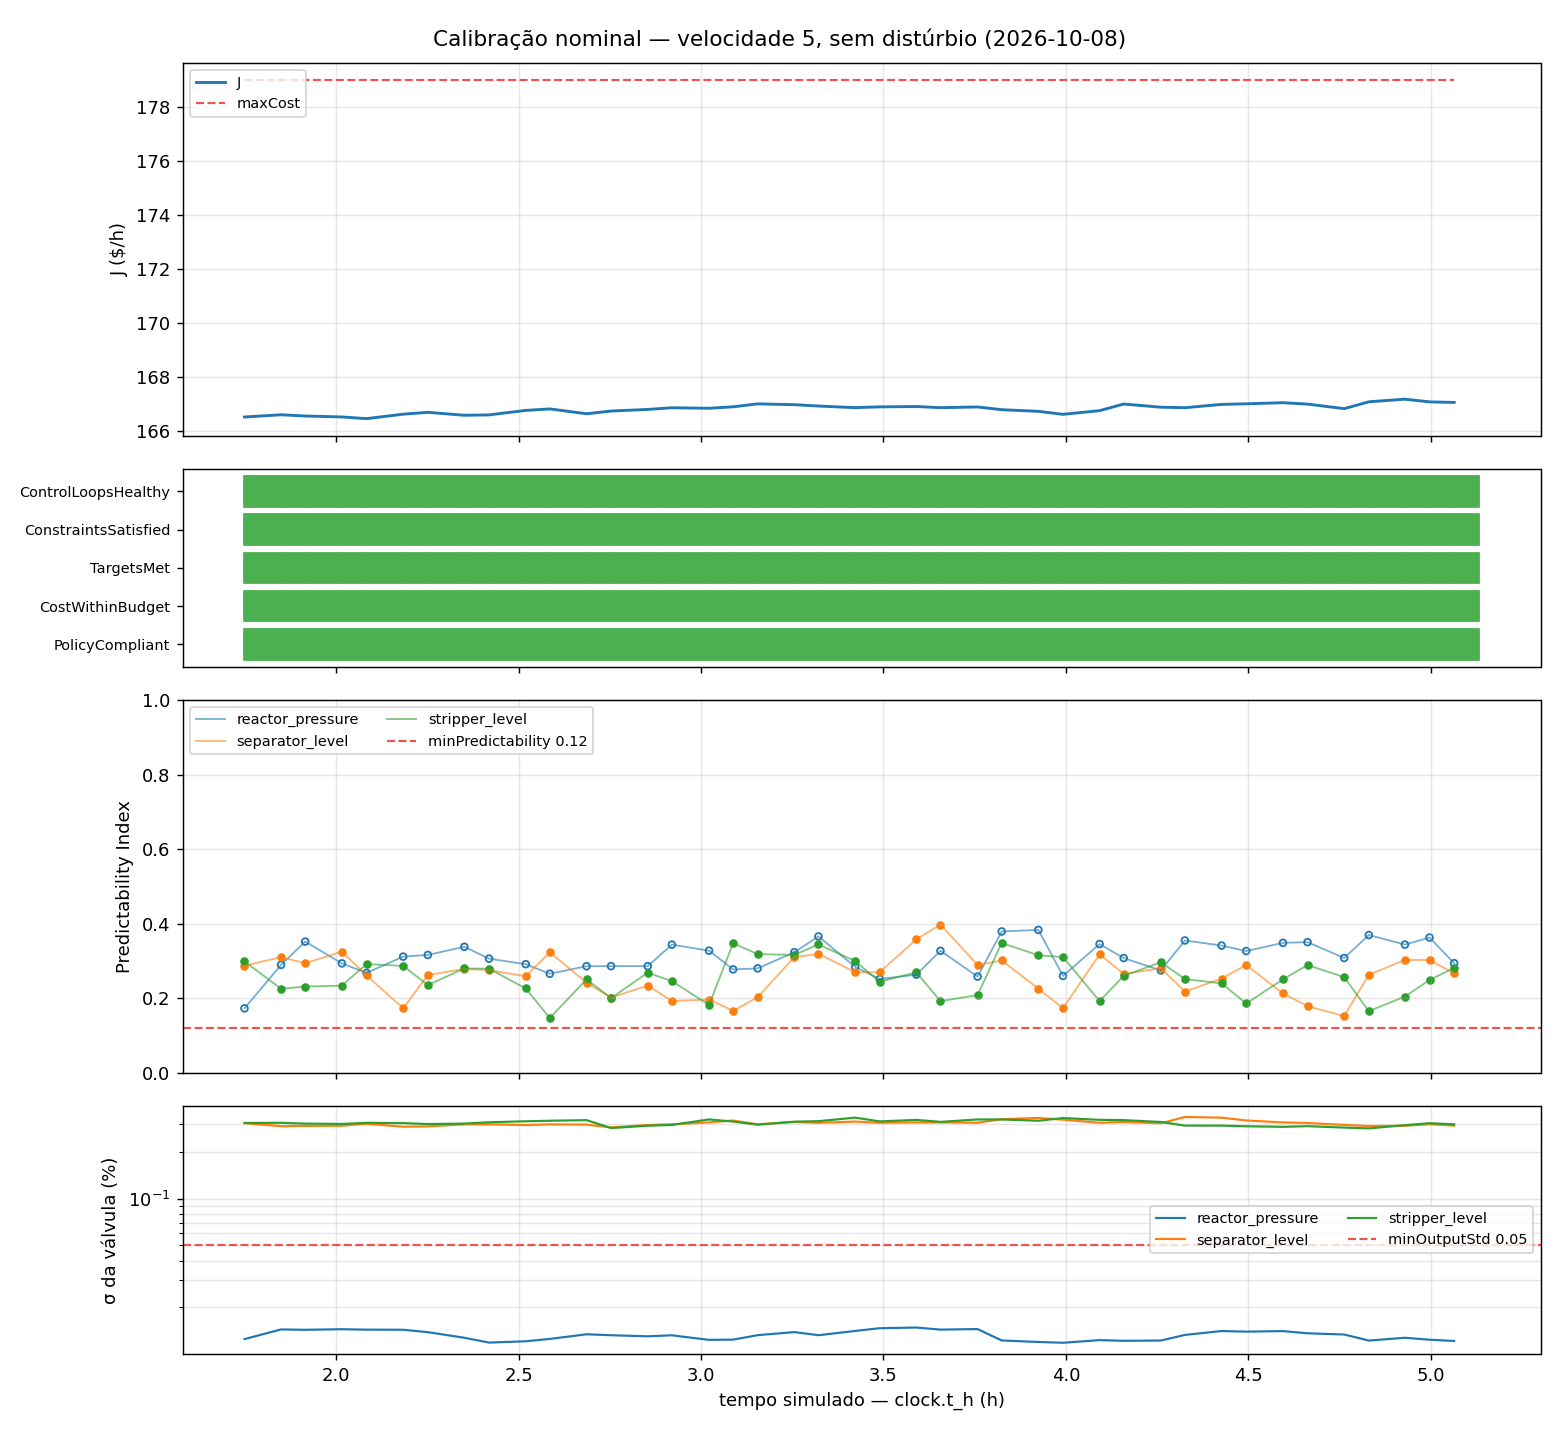
\includegraphics[width=\textwidth]{imagens/tep-exp-calibracao.png}
	\fonte{Elaborado pelo autor.}
	\label{fig:calibracao}
\end{figure}

Desses números saíram os valores da política (Seção~\ref{subsec:politica_modo1}): o orçamento de 170,6~\$/h, o custo do caso base, cerca de 2,3~\% acima do custo medido; o limite de 0,12 para o índice, abaixo do menor valor nominal, com folga; e o \textit{offset} máximo de 20~kPa e 1~\%, acima dos máximos nominais.

A rodada de controle do Experimento~27, de 40~h, mostrou um problema nessa calibração. Com as malhas proporcionais, a planta não estava em regime no começo das rodadas: ela converge por dezenas de horas, e o custo sobe junto, de 166,3 para 169,8~\$/h, a menos de 1~\$/h do orçamento (Tabela~\ref{tab:controle_p}). O custo de referência foi medido entre 1,75 e 5,06~h, no início desse transitório. O veredito foi \texttt{Compliant} nas 84 avaliações, mas o custo ainda subia no fim da rodada, cerca de 0,04~\$/h por hora, e, numa rodada mais longa, o orçamento pode estourar sem distúrbio nenhum. O orçamento precisa ser recalibrado com o custo de regime. Isso não invalida as rodadas com o IDV(6) da Seção~\ref{sec:sup_idv6}: no trecho em que elas foram feitas, a deriva nominal do custo é de cerca de 0,2~\$/h por hora, muito menor que o efeito do distúrbio.

\FloatBarrier
% -------------------------------------------------------------------------
\section{O supervisor sob distúrbio}
\label{sec:sup_idv6}

O distúrbio escolhido foi o IDV(6), a perda da alimentação de A, um dos cinco implementados (Seção~\ref{subsec:disturbios}). Sem A, as reações que produzem G e H desaceleram, os outros reagentes se acumulam no reciclo, a pressão do reator sobe e a purga abre, levando mais reagente caro. A expectativa era que a vazão de produto caísse, que o custo subisse até estourar o orçamento e que o supervisor declarasse \texttt{NonCompliant} depois de três avaliações ruins seguidas, sem nenhuma mudança na política. A Tabela~\ref{tab:idv6} resume as duas rodadas com o distúrbio.

\begin{table}[htbp]
	\centering
	\caption{Eventos nas rodadas com o IDV(6), contados a partir do instante em que o distúrbio foi ligado.}
	\label{tab:idv6}
	\footnotesize
	\begin{tabular}{|>{\raggedright\arraybackslash}p{0.5\textwidth}|c|c|}
		\hline
		\textbf{Evento} & \textbf{Experimento 25} & \textbf{Experimento 26} \\
		\hline
		Níveis do separador e do \textit{stripper} passam do \textit{offset} máximo & sem o critério & +0,84~h \\
		\texttt{TargetsMet} False (vazão de produto abaixo da meta) & +0,98~h & +0,94~h \\
		\texttt{ControlLoopsHealthy} False & não virou & +1,00~h \\
		\texttt{CostWithinBudget} False e fase \texttt{NonCompliant} & +1,15~h & +1,11~h \\
		Pressão do reator passa do \textit{offset} máximo & sem o critério & +1,44~h \\
		IDV(6) desligado & +1,53~h & +1,20~h \\
		Custo no fim da gravação & 218,2~\$/h & 195,2~\$/h \\
		\hline
	\end{tabular}
	\fonte{Elaborado pelo autor, a partir das gravações dos Experimentos~25 e~26.}
\end{table}

\subsection{Experimento 25: o veredito econômico}
\label{subsec:exp25}

O veredito virou na ordem física esperada: primeiro a vazão de produto, depois o custo (Figura~\ref{fig:exp25}). Logo depois do distúrbio, o custo até caiu um pouco, de 166,5 para 165,0~\$/h, porque sai menos A na purga. Depois, a vazão de produto ficou abaixo do mínimo de 21,80~m$^3$/h em +0,98~h, e o custo estourou o orçamento em +1,15~h, já na terceira avaliação ruim seguida, levando a fase a \texttt{NonCompliant}. Do distúrbio ao veredito passaram 1,15~h de processo, cerca de 7 minutos de relógio. Os limites não foram violados, mas chegaram perto: a pressão do reator subiu de cerca de 2695 para 2840~kPa, contra o limite de 2895~kPa, e o nível do reator, de 72 para 90~\%.

\begin{figure}[htbp]
	\centering
	\caption{Experimento 25, IDV(6) com a política fixa: custo, \textit{conditions}, índice das malhas na escala do código e desvio padrão das válvulas.}
	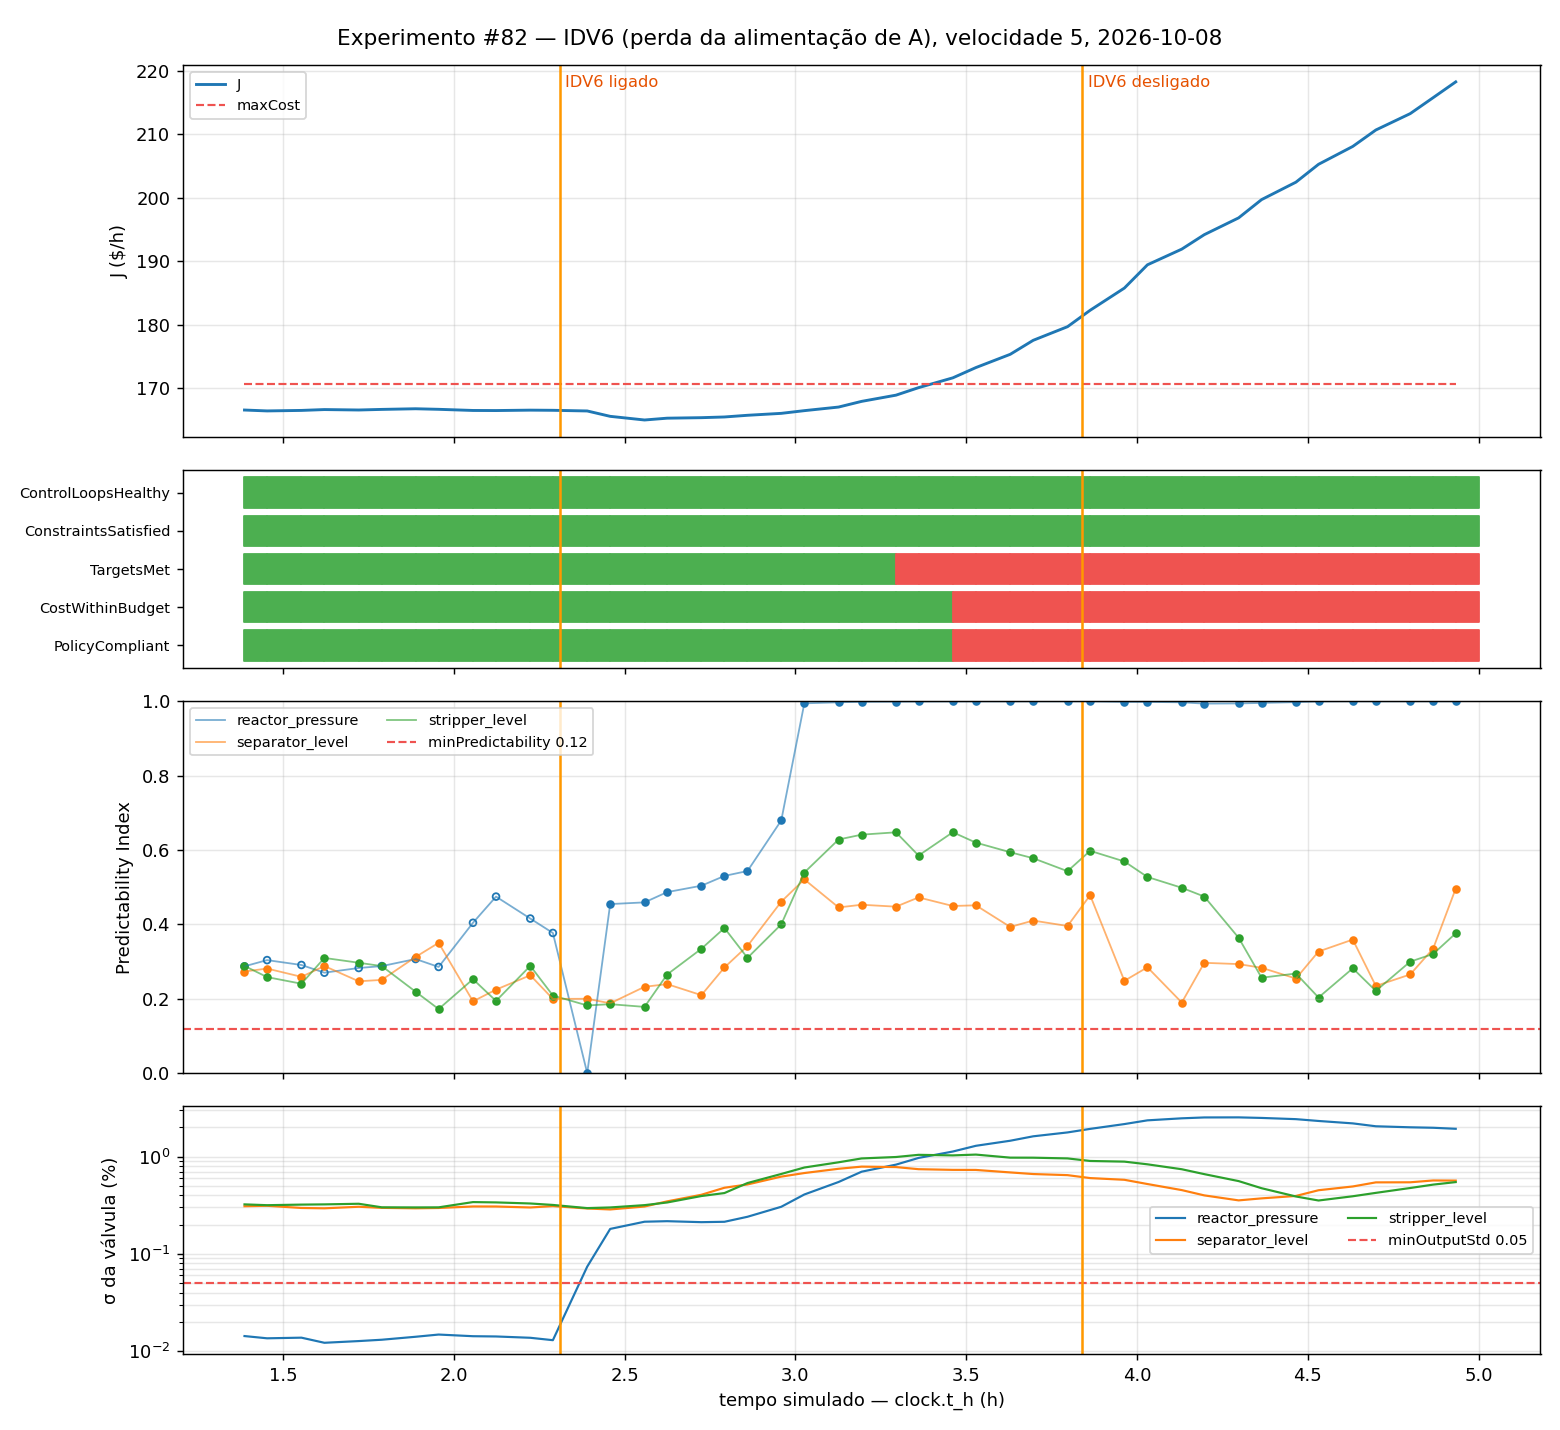
\includegraphics[width=\textwidth]{imagens/tep-exp25-idv6.png}
	\fonte{Elaborado pelo autor.}
	\label{fig:exp25}
\end{figure}

Quando o IDV(6) foi desligado, a planta não voltou: a pressão, o nível e o custo continuaram subindo até o fim da gravação. O nível do reator não tem malha, a malha de pressão é só proporcional, e os reagentes acumulados no reciclo saem devagar pela purga.

No nível das malhas, o supervisor não viu nada: \texttt{ControlLoopsHealthy} ficou True nas 44 avaliações. A malha de pressão passou a ser julgada assim que a purga começou a se mexer e teve uma única avaliação abaixo do limite, no instante do degrau, que a persistência segurou. Depois disso, o índice dela foi a cerca de 1,0 e ficou ali, com a pressão até 131~kPa acima do \textit{setpoint}. Na escala do código, um índice perto de 1 é lido como malha saudável. A Seção~\ref{sec:releitura_pi} volta a esse ponto.

\subsection{Experimento 26: o critério de seguimento}
\label{subsec:exp26}

O índice de \citeonline{Bradu2018} supõe que a malha segue o \textit{setpoint} em média, e o sistema do CERN já tinha alarmes de desvio, que o índice complementa. O laboratório não tinha esse alarme. O critério \texttt{maxOffset} foi acrescentado ao supervisor e à política (Seção~\ref{subsec:veredito}), com 20~kPa para a pressão e 1~\% para os níveis, e a rodada foi repetida nas mesmas condições (Figura~\ref{fig:exp26}).

Os níveis do separador e do \textit{stripper} passaram do \textit{offset} máximo 0,84~h depois do distúrbio, com índices de 0,44 e 0,55, que pelo índice sozinho seriam saudáveis. A vazão de produto saiu da meta em +0,94~h, \texttt{ControlLoopsHealthy} virou False em +1,00~h, e o \texttt{NonCompliant} veio em +1,11~h. A pressão passou do \textit{offset} máximo depois, em +1,44~h. De novo, a planta não se recuperou depois que o distúrbio foi desligado.

\begin{figure}[htbp]
	\centering
	\caption{Experimento 26, a mesma rodada com o critério de seguimento do \textit{setpoint}: custo, \textit{conditions}, índice das malhas na escala do código e desvio padrão das válvulas.}
	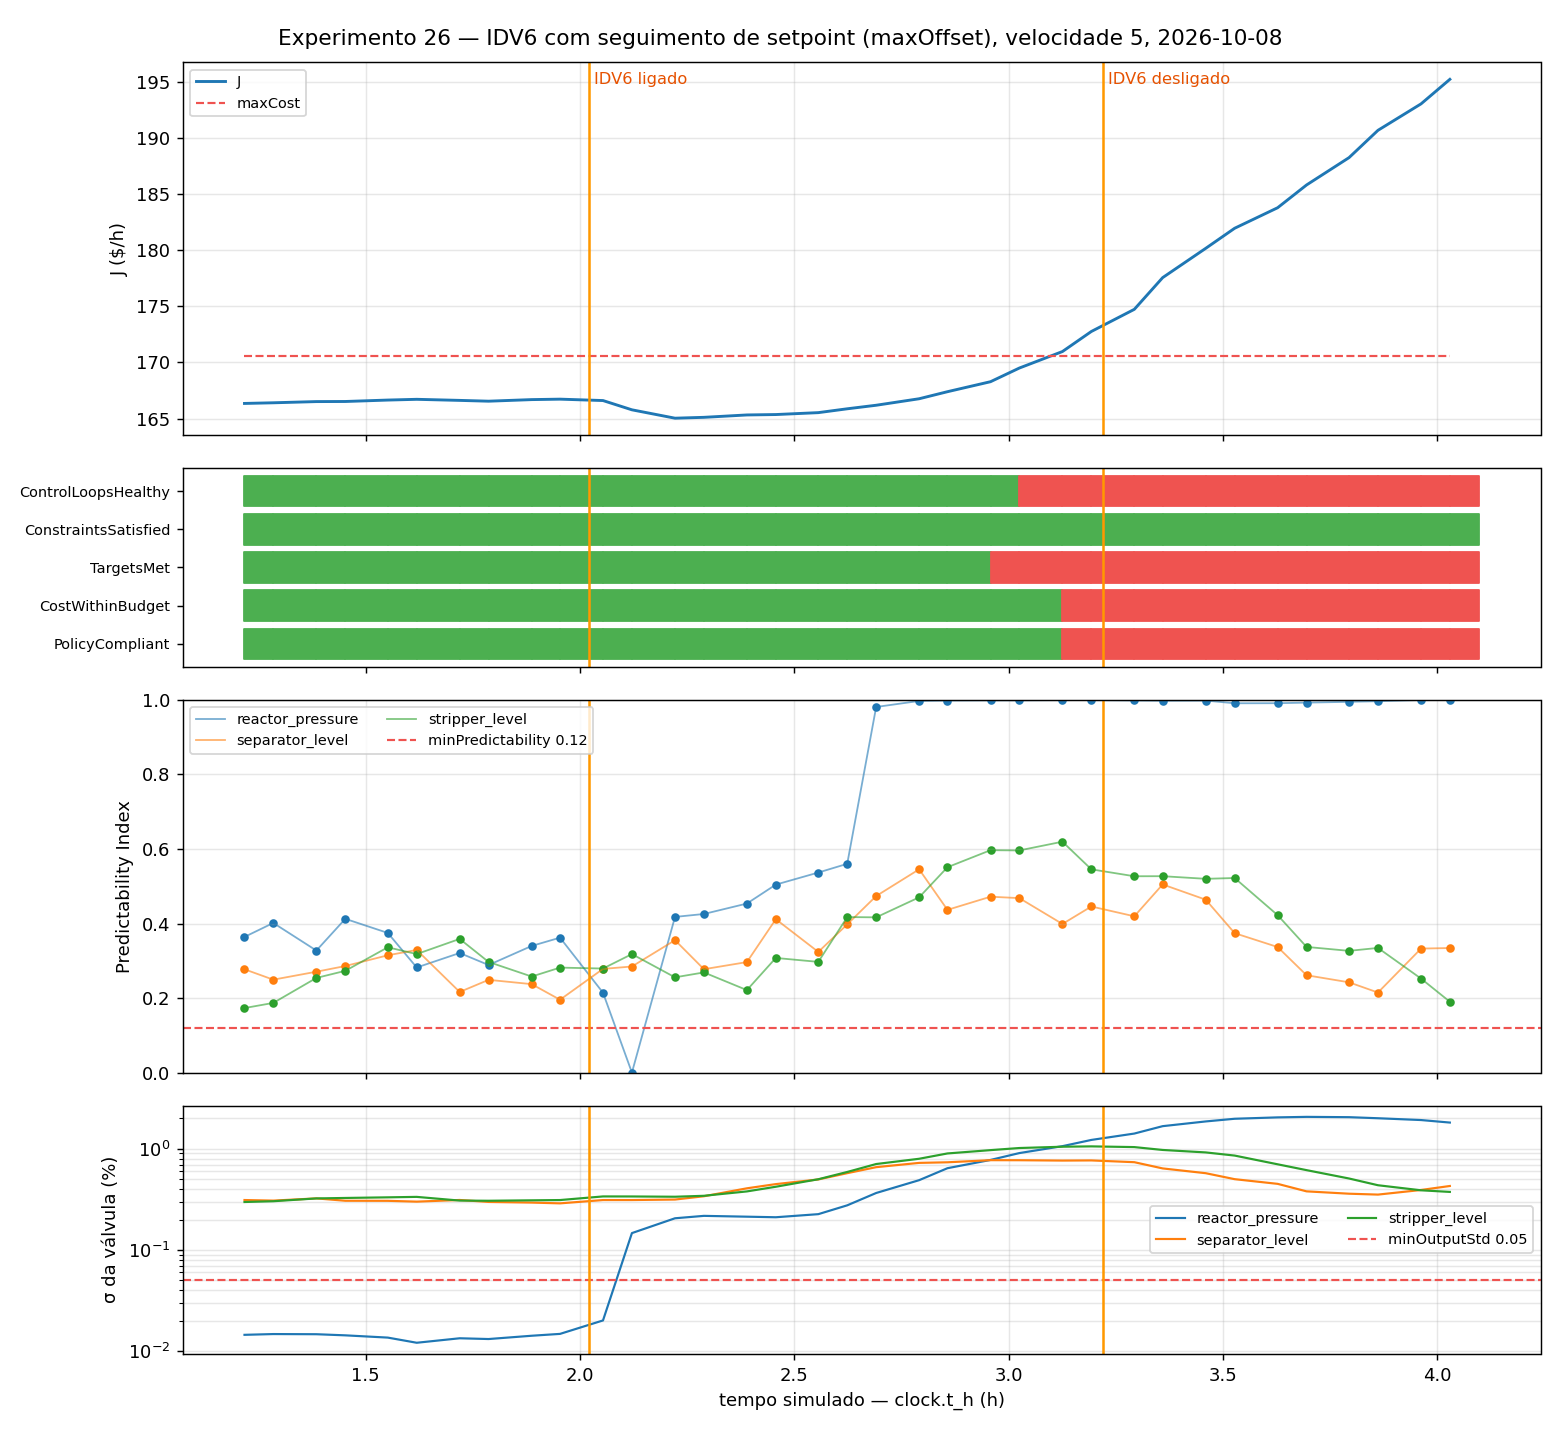
\includegraphics[width=\textwidth]{imagens/tep-exp26-idv6-maxoffset.png}
	\fonte{Elaborado pelo autor.}
	\label{fig:exp26}
\end{figure}

Com o critério de seguimento, o supervisor passou a mostrar a degradação na ordem em que ela acontece: as malhas de nível perdem o alvo primeiro, a vazão de produto cai em seguida, e o custo estoura por último. Quem detectou foi o seguimento, e não o índice.

\FloatBarrier
% -------------------------------------------------------------------------
\section{Malhas PI em operação normal}
\label{sec:sup_pi}

Os Experimentos~25 e~26 mostraram que, com as malhas proporcionais, a planta não volta do IDV(6). A ação integral parecia o remédio, porque uma malha PI não aceita \textit{offset} permanente. As três malhas passaram a PI, na versão 2.1.0-alpha (Seção~\ref{subsec:malhas}), e, antes de repetir o IDV(6), a planta foi rodada sem distúrbio, para achar o novo ponto de operação e o novo custo de referência. Foram três rodadas (Tabela~\ref{tab:rodadas}): duas com PI, às velocidades 5 e 30, e uma de controle, com o mesmo código, a não ser pela integral congelada, o que deixa as malhas iguais às proporcionais.

Na rodada 1, as malhas PI fizeram o que deviam. O \textit{offset} da pressão foi de 9,7~kPa a zero em cerca de 3,8~h, sem oscilação sustentada, e os níveis ficaram a menos de 0,33~\% do \textit{setpoint}. Mas o custo não assentou: caiu de 166,9 para 151,4~\$/h em 10~h e continuava caindo.

A rodada 2, mais longa, mostrou o porquê (Tabela~\ref{tab:exp27} e Figura~\ref{fig:exp27_sinais}). A pressão ficou a poucos kPa do \textit{setpoint}, mas, para mantê-la ali, o controlador foi fechando a purga cada vez mais rápido, de 38,7 para 17,8~\% em 30~h. Com menos purga, o inerte B se acumulou, e o nível do reator, que não tem malha, foi caindo, de 71,6 para 47,8~\%. Em $t \approx 31$~h, o nível cruzou 45,8~\%, o ponto em que, no próprio \texttt{teprob.f}, o coeficiente de troca térmica do reator começa a cair com o nível, porque o feixe de resfriamento fica descoberto. A temperatura subiu de 120,5 para 133,8~°C em 1,6~h, a purga saturou fechada e, em $t = 32{,}9$~h, a pressão passou de 3000~kPa, o limite de parada de emergência. Na rodada de controle, a mesma planta, com as malhas proporcionais, convergiu em 40~h.

\begin{table}[htbp]
	\centering
	\caption{A planta com as malhas PI, sem distúrbio, na rodada 2 do Experimento~27.}
	\label{tab:exp27}
	\scriptsize
	\begin{tabular}{|c|c|c|c|c|c|c|c|}
		\hline
		\textbf{$t$ (h)} & \cabecalho{\textbf{Purga}\\\textbf{(\%)}} & \cabecalho{\textbf{Pressão}\\\textbf{(kPa)}} & \cabecalho{\textbf{Nível do}\\\textbf{reator (\%)}} & \cabecalho{\textbf{B na purga}\\\textbf{(\% mol)}} & \cabecalho{\textbf{T do}\\\textbf{reator (°C)}} & \cabecalho{\textbf{Produto}\\\textbf{(m$^3$/h)}} & \cabecalho{\textbf{$J$}\\\textbf{(\$/h)}} \\
		\hline
		0,4 & 38,7 & 2695,3 & 71,6 & 14,37 & 120,44 & 22,98 & 165,9 \\
		10 & 33,8 & 2703,1 & 69,5 & 14,95 & 120,46 & 23,10 & 152,1 \\
		20 & 27,5 & 2702,3 & 63,1 & 16,23 & 120,50 & 23,26 & 133,3 \\
		30 & 17,8 & 2701,6 & 47,8 & 18,93 & 120,54 & 23,58 & 105,3 \\
		31,0 & 16,8 & 2701,0 & 45,6 & 19,29 & 120,69 & 23,59 & 102,6 \\
		32,0 & 4,3 & 2646,8 & 41,3 & 20,49 & 124,02 & 24,80 & -- \\
		32,6 & 0,0 & 2548,2 & 30,5 & 22,85 & 133,84 & 28,05 & 74,6 \\
		32,9 & 41,9 & 3029,3 & 13,1 & -- & 105,99 & 28,94 & 55,1 \\
		\hline
	\end{tabular}
	\fonte{Elaborado pelo autor, a partir do registro do Experimento~27.}
\end{table}

\begin{figure}[htbp]
	\centering
	\caption{Experimento 27: as rodadas inteiras com as malhas PI (azul, até a perda da planta) e com as malhas proporcionais (verde, 40~h), nos mesmos eixos.}
	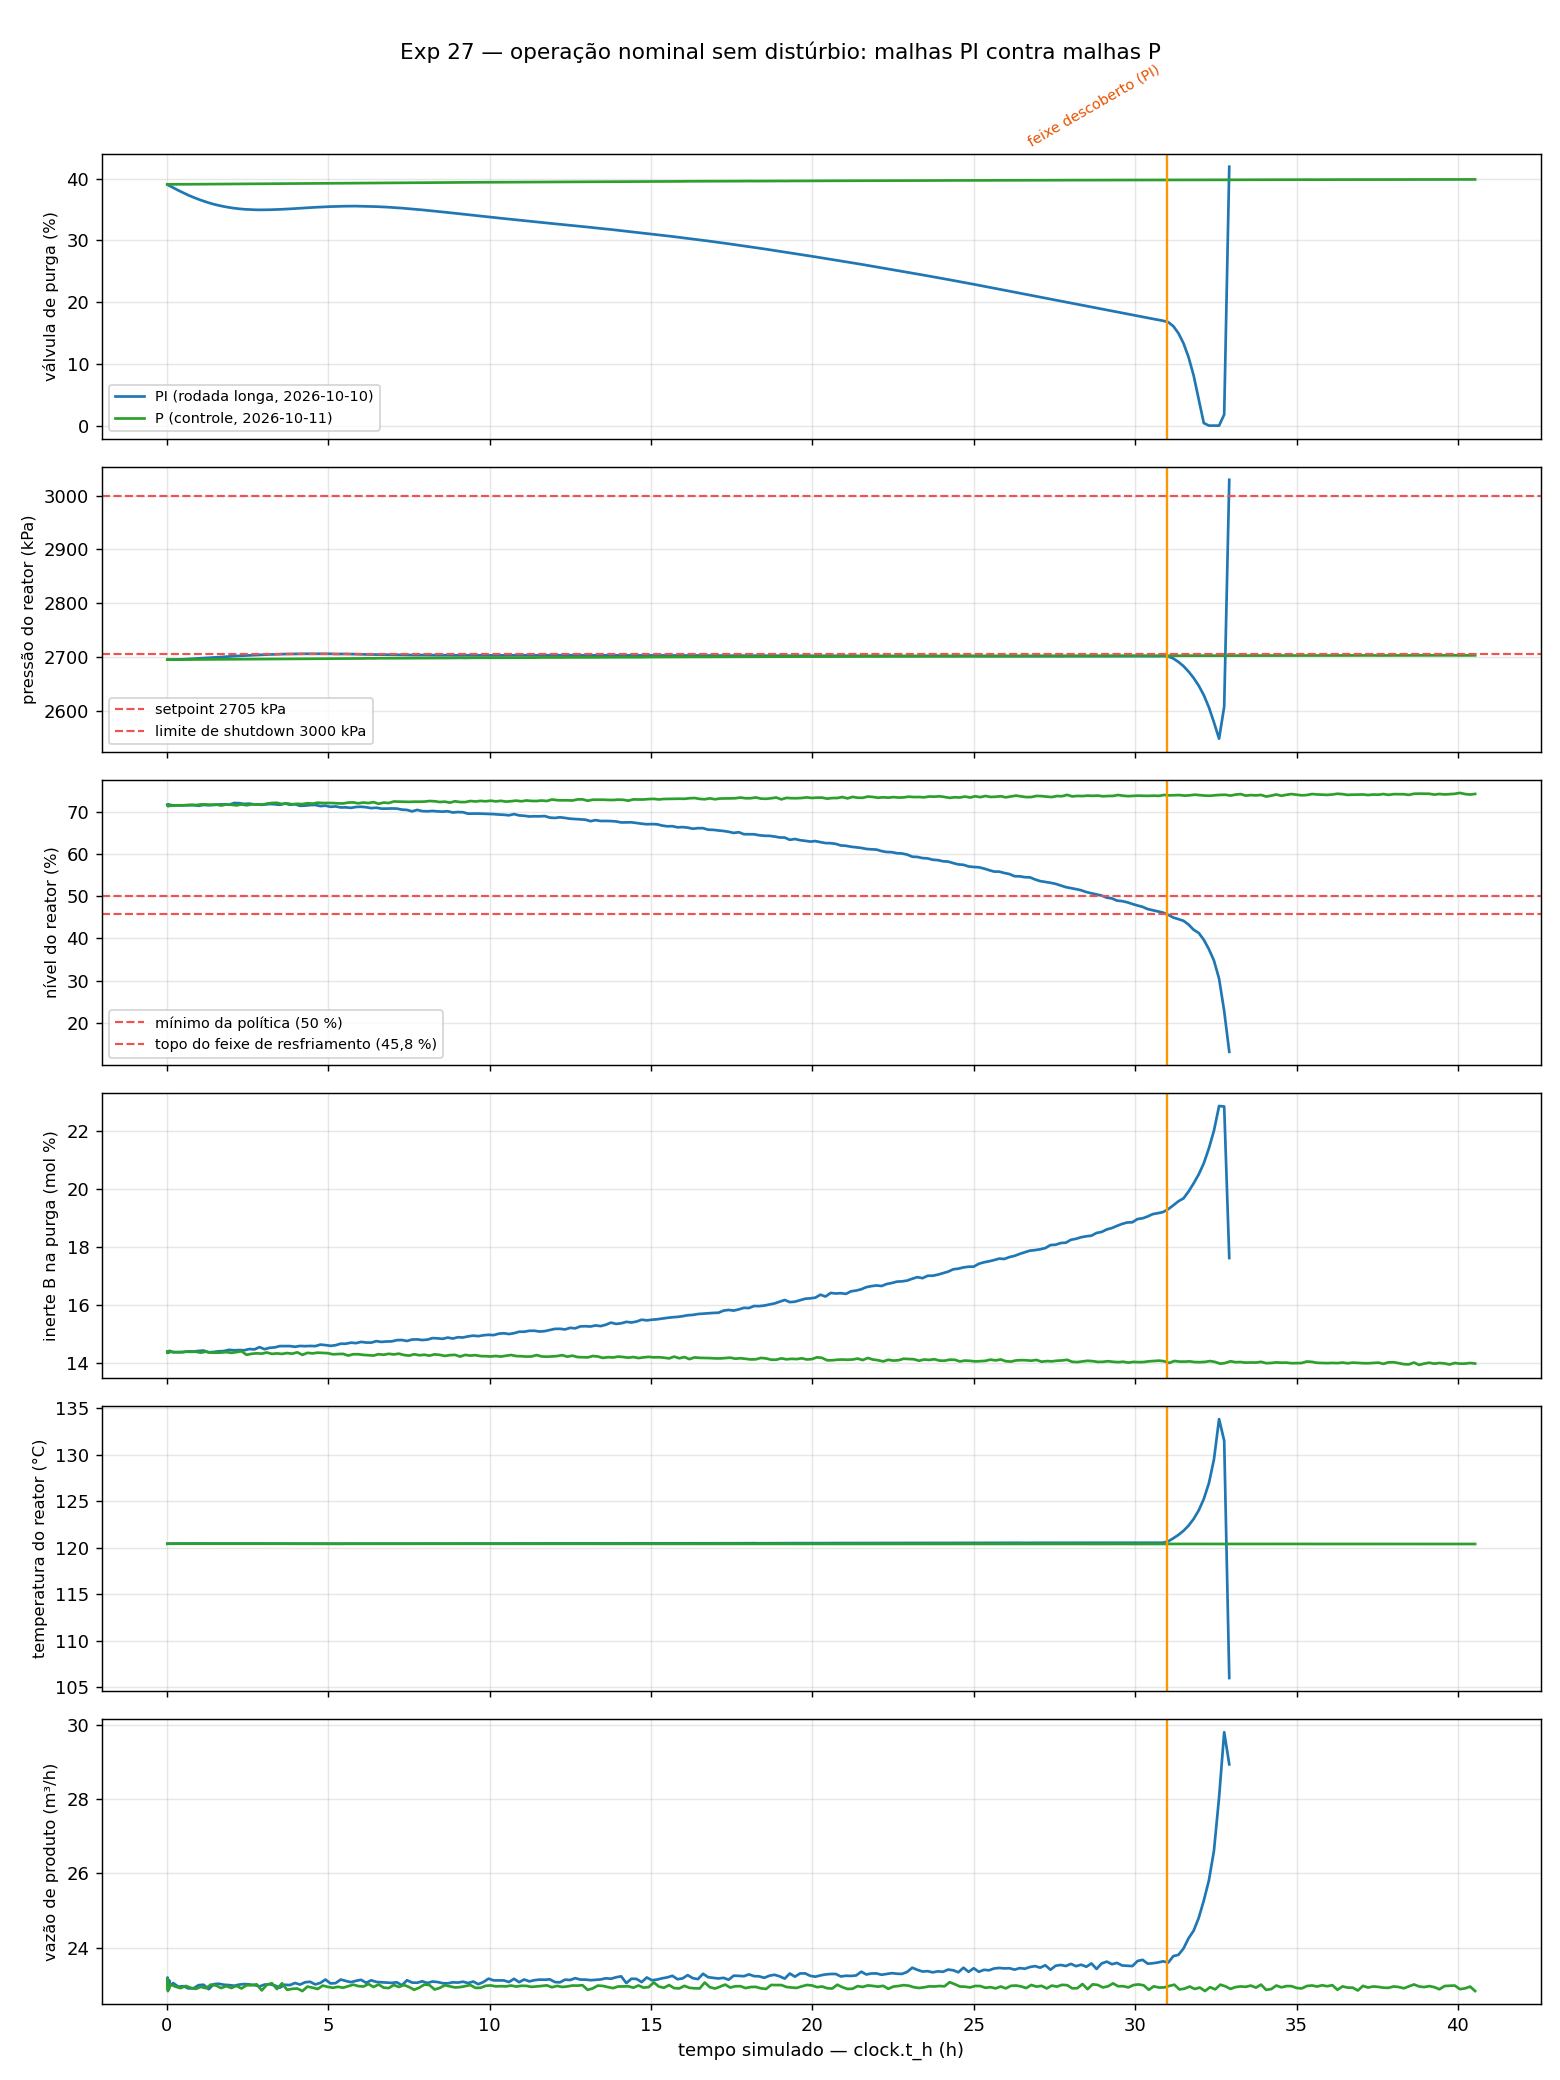
\includegraphics[width=\textwidth,height=0.78\textheight,keepaspectratio]{imagens/tep-exp27-pi-vs-p.png}
	\fonte{Elaborado pelo autor.}
	\label{fig:exp27_sinais}
\end{figure}

O registro do experimento propõe uma explicação, que é uma leitura dos dados e não algo provado. Com a malha proporcional, a pressão pode estacionar fora do \textit{setpoint}, e essa folga deixa a planta se ajustar: a pressão sobe alguns kPa, o nível do reator sobe um pouco, e tudo para. Com a integral, a pressão fica presa no \textit{setpoint}, e quem absorve o desbalanço é a purga, que decide quanto gás sai, mas não quanto líquido fica no reator. O que está provado é que, na mesma planta, com o mesmo ruído e a mesma velocidade, as malhas proporcionais convergem e as PI divergem. O teste direto da leitura, com PI só nas malhas de nível, ficou pendente.

O que o supervisor viu está na Figura~\ref{fig:exp27_sup}. O custo caiu o tempo todo, de 165,9 para 55,1~\$/h, e \texttt{CostWithinBudget} ficou True nas 70 avaliações. Menos purga significa menos reagente perdido na conta de Downs e Vogel, então o custo ``melhorou'' enquanto a planta consumia o próprio inventário. As malhas também ficaram saudáveis até o fim, pelos dois testes: de 6 a 31~h, o \textit{offset} da pressão não passou de 3,4~kPa, e o dos níveis, de 0,27~\%. O problema estava numa variável que não tem malha.

\begin{figure}[htbp]
	\centering
	\caption{Experimento 27, rodada 2: o que o supervisor viu. Custo, \textit{conditions}, índice das malhas na escala do código, \textit{offset} dividido pelo máximo da política e desvio padrão das válvulas.}
	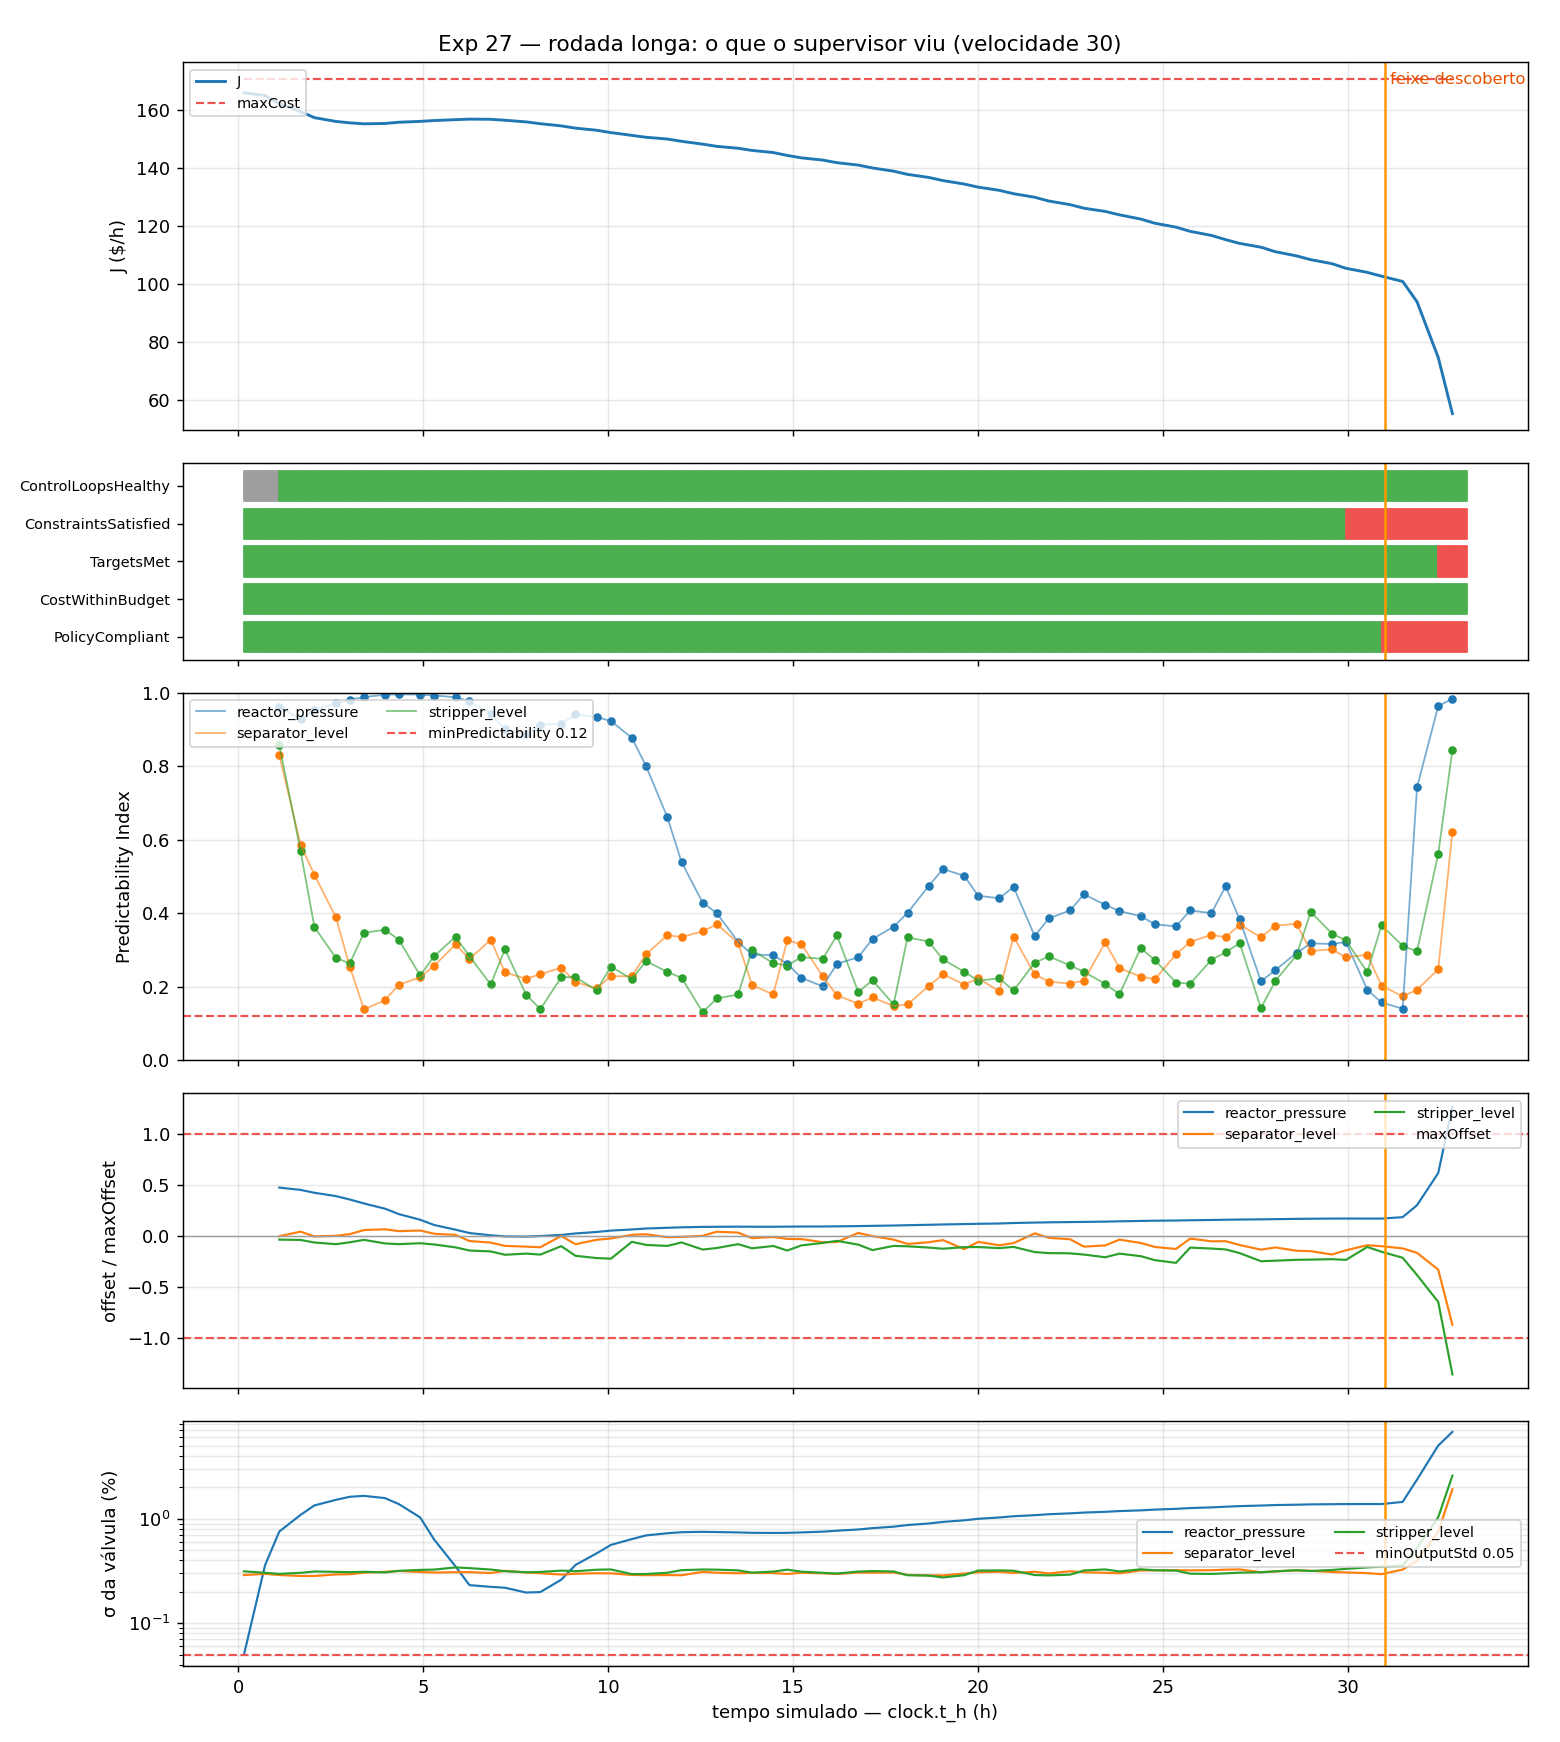
\includegraphics[width=\textwidth,height=0.78\textheight,keepaspectratio]{imagens/tep-exp27-supervisor.png}
	\fonte{Elaborado pelo autor.}
	\label{fig:exp27_sup}
\end{figure}

Quem percebeu foi o limite de nível do reator declarado na política, de no mínimo 50~\%. O nível cruzou esse valor em $t \approx 29{,}1$~h, \texttt{ConstraintsSatisfied} virou False em 29,96~h, e o \texttt{NonCompliant} veio em 30,92~h, praticamente junto com o início da perda física. Parte desse atraso vem da velocidade 30, em que cada avaliação cobre cerca de 28 minutos de processo. Mesmo assim, o aviso foi tarde: o nível caiu por 25~h dentro da faixa permitida antes de cruzar o limite. Um limite fixo avisa quando a variável chega lá, e não quando ela começa a ir.

Depois desse experimento, o ramo principal do \texttt{tep-plant} ficou com as malhas PI, ou seja, com a planta que se perde em cerca de 33~h sem distúrbio. A escolha entre criar a malha de nível do reator e voltar a pressão para proporcional ficou para depois deste trabalho.

\FloatBarrier
% -------------------------------------------------------------------------
\section{A escala do índice das malhas}
\label{sec:releitura_pi}

A Seção~\ref{subsec:indice_malhas} mostrou que o código calcula o índice na escala contrária à da leitura adotada na Seção~\ref{sec:diagnostico}. Para ver o que muda, os julgamentos das malhas foram refeitos sobre as gravações, sem rodar a planta de novo. O \textit{historian} limita o índice ao intervalo de 0 a 1, e, dentro dele, o índice na escala do artigo é 1 menos o gravado. Nas poucas avaliações em que o gravado vale 0, o da escala do artigo vale 1 ou mais, o que não muda o julgamento. O limite foi calibrado do mesmo jeito que o 0,12 da política: na rodada nominal, o índice na escala do artigo ficou entre 0,60 e 0,85, e o limite foi posto em 0,5. O portão de 0,05~\% e a persistência de três avaliações são os mesmos do supervisor. O critério de \textit{offset} ficou de fora, para isolar o efeito do índice.\footnote{O cálculo é o comando \texttt{loop-rereading}, do pacote de análise em \texttt{tep-lab/analysis}. O comando exato que gera a figura e a tabela desta seção está em \texttt{tep-lab/data/README.md}.} A Tabela~\ref{tab:releitura} mostra o resultado.

\begin{table}[htbp]
	\centering
	\caption{Julgamento das malhas refeito na escala do artigo, comparado com o que o supervisor fez.}
	\label{tab:releitura}
	\footnotesize
	\begin{tabular}{|>{\raggedright\arraybackslash}p{0.27\textwidth}|>{\raggedright\arraybackslash}p{0.17\textwidth}|c|>{\raggedright\arraybackslash}p{0.27\textwidth}|}
		\hline
		\textbf{Rodada} & \textbf{Primeiro alarme} & \cabecalho{\textbf{Avaliações}\\\textbf{com alarme}} & \textbf{O que o supervisor fez} \\
		\hline
		Calibração (P, velocidade 5) & nenhum & 0~\% & nenhum alarme \\
		Experimento 25 (P, velocidade 5, IDV(6)) & 2,86~h (+0,55~h) & 59~\% & malhas nunca sinalizadas; \texttt{NonCompliant} em +1,15~h \\
		Experimento 26 (P, velocidade 5, IDV(6)) & 2,62~h (+0,60~h) & 51~\% & malhas sinalizadas pelo \textit{offset} em +1,00~h \\
		Exp. 27, rodada 1 (PI, velocidade 5) & 0,46~h & 29~\% & nenhum alarme \\
		Exp. 27, rodada 2 (PI, velocidade 30) & 2,07~h & 33~\% & \texttt{NonCompliant} pelo nível do reator em 30,92~h \\
		Exp. 27, controle (P, velocidade 30) & 5,34~h & 4~\% & nenhum alarme \\
		\hline
	\end{tabular}
	\fonte{Elaborado pelo autor, a partir das gravações em \texttt{tep-lab/data}.}
\end{table}

Na escala do artigo, o índice teria sinalizado o IDV(6) cerca de 0,6~h depois do distúrbio, antes do veredito econômico e antes do critério de \textit{offset}. Quem dispara é a malha de pressão: sob o distúrbio, o erro dela vira uma deriva lenta, que o modelo autorregressivo prevê quase toda, e o índice cai a perto de zero (Figura~\ref{fig:releitura}). É o comportamento que \citeonline{Bradu2018} descrevem: um erro previsível indica que há algo a melhorar na malha. Na operação nominal, à velocidade 5, nenhuma malha foi sinalizada.

\begin{figure}[htbp]
	\centering
	\caption{Índice das malhas na escala do artigo, com o limite recalibrado. As faixas vermelhas são os trechos em que \texttt{ControlLoopsHealthy} teria ficado False. Pontos vazados são avaliações em que a malha não seria julgada, abaixo do portão.}
	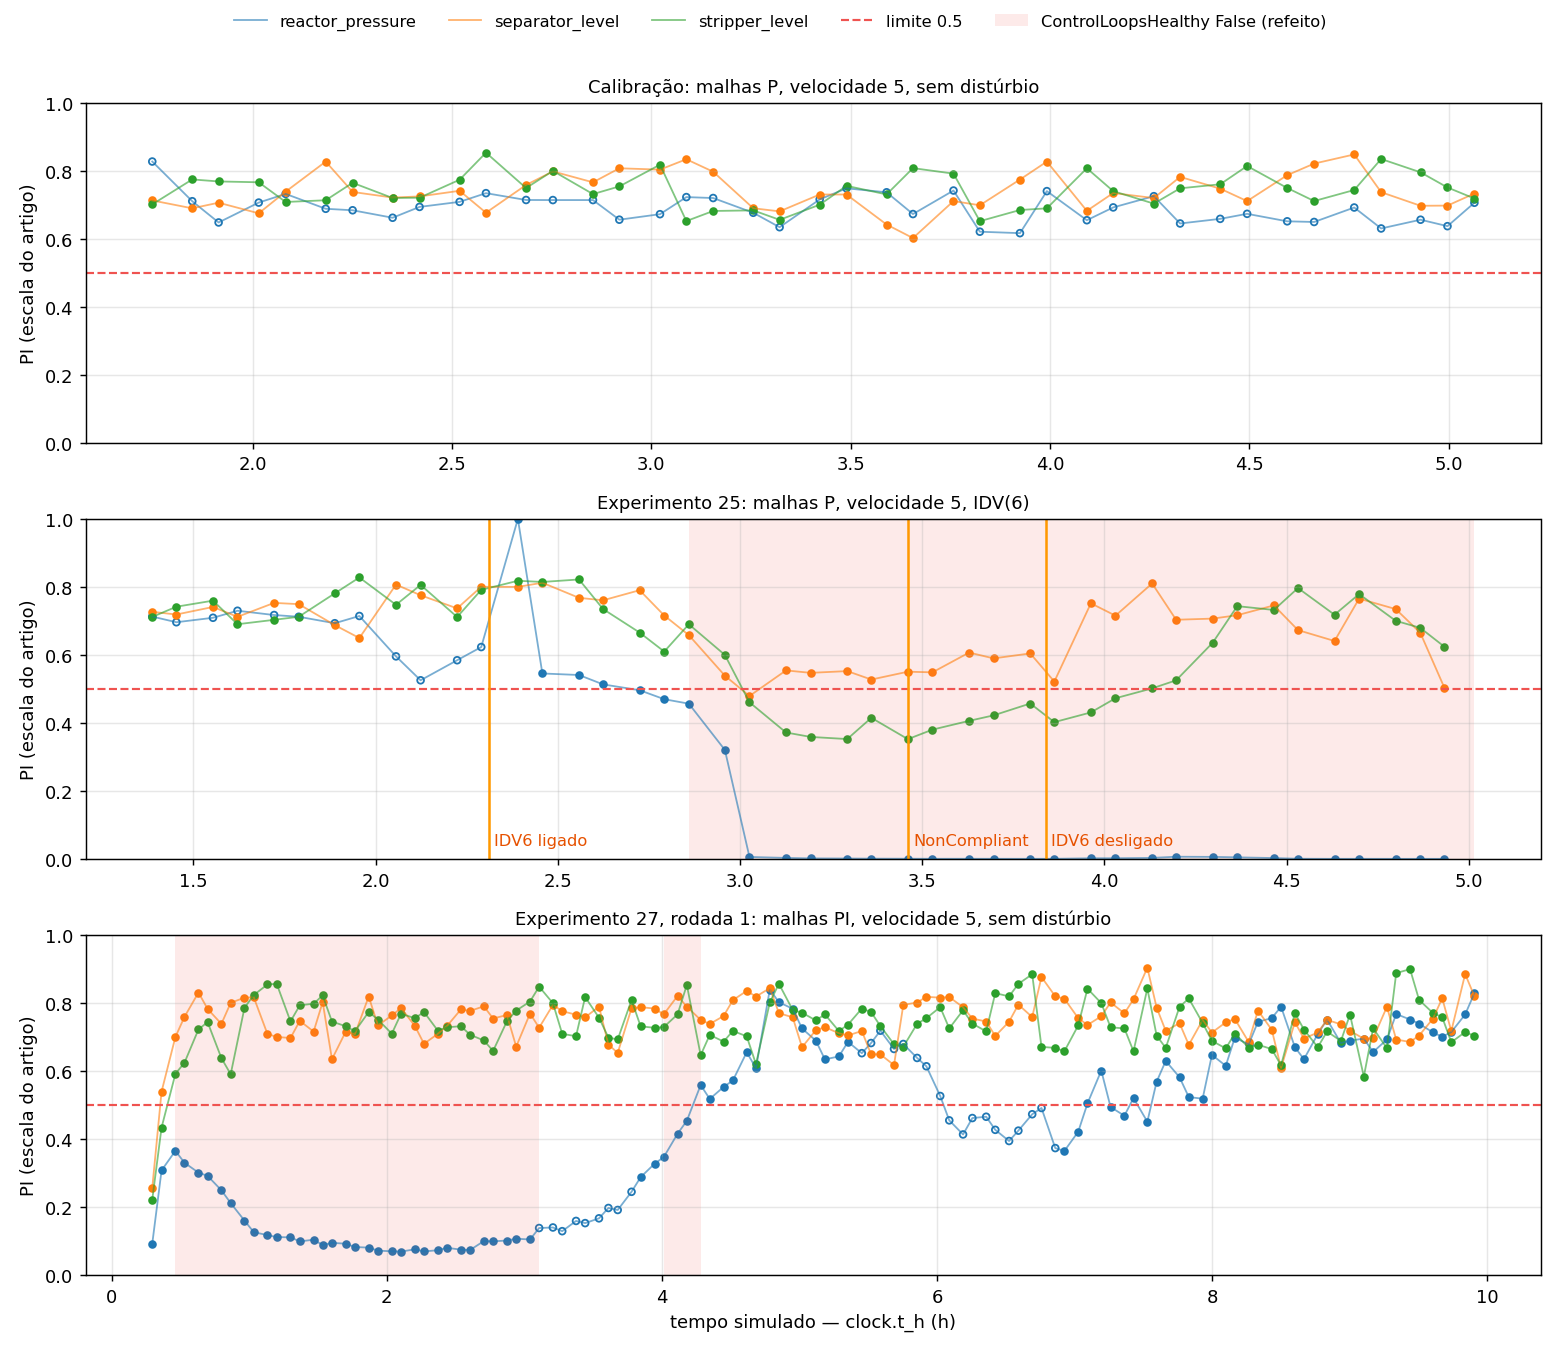
\includegraphics[width=\textwidth]{imagens/tep-releitura-pi.png}
	\fonte{Elaborado pelo autor.}
	\label{fig:releitura}
\end{figure}

O mesmo índice, porém, também sinaliza o que não é problema. Na rodada 1 do Experimento~27, ele sinalizou a malha de pressão de 0,46 a cerca de 3~h, enquanto o PI levava a pressão ao \textit{setpoint}: um transitório suave e intencional, e por isso previsível. Nas rodadas à velocidade 30, em que a janela de 300~s cobre cerca de 4,7~h de processo, as derivas lentas de pressão e de nível também viraram alarme, inclusive na rodada de controle, com a planta estável. O índice responde a qualquer erro previsível, sem distinguir um distúrbio de um transitório esperado, e o tamanho da janela, medida em tempo de relógio, muda o que ele enxerga.

Duas conclusões saem daí. A escala do código deixou o índice cego justamente para o caso que o Experimento~25 queria detectar; na escala certa, ele teria detectado. E, mesmo na escala certa, o índice serve como complemento do critério de \textit{offset} e dos limites da política, como no CERN, e não como substituto. Esta é uma releitura de dados gravados: o código do \textit{historian} e do supervisor não foi alterado, e corrigir a escala exige também recalibrar o limite e medir as janelas em tempo simulado.

\FloatBarrier
% -------------------------------------------------------------------------
\section{Discussão}
\label{sec:discussao_resultados}

Os resultados permitem voltar aos objetivos específicos do Capítulo~1, um a um.

O primeiro objetivo era colocar o TEP para rodar como uma planta contínua, exposta por OPC~UA, e verificar que ela se comporta como o modelo original. Nos dois testes em regime, a planta reproduziu o modelo: no caso base, as derivadas ficaram perto de zero e as medições e o custo bateram com os valores publicados, e, na versão com a água de resfriamento integrada, o ótimo do Modo~1 de Ricker foi reencontrado. Em operação, com as malhas proporcionais, ela se aproxima devagar do caso base. As diferenças conhecidas são a água de resfriamento constante nas versões usadas com o supervisor, os analisadores contínuos e os distúrbios aleatórios, que ainda faltam.

O segundo objetivo era o \textit{historian}. Ele coletou os sinais a cada 100~ms e respondeu ao supervisor em todas as rodadas. A janela medida em tempo de relógio, porém, fez as rodadas à velocidade 30 enxergarem horas de processo numa janela só, e esse efeito apareceu no Experimento~27.

O terceiro objetivo era declarar a política do Modo~1 no Kubernetes sem que o supervisor precisasse conhecer o TEP. A política foi declarada como manifestos, e o código do supervisor não tem nada do TEP: o orçamento, as metas, os limites e os critérios das malhas foram ajustados só nos manifestos. Há uma ressalva. Acrescentar um tipo novo de critério, como o \textit{offset} máximo, exigiu um campo novo no código do supervisor. A política é declarativa dentro do vocabulário que o supervisor conhece.

O quarto objetivo era verificar que o veredito acompanha a planta, em operação normal e sob distúrbio, com a política fixa. O veredito ficou \texttt{Compliant} em operação normal, virou \texttt{NonCompliant} sob o IDV(6), na ordem física dos acontecimentos, e ficou assim enquanto a planta não se recuperou. Já a deriva do Experimento~27 foi pega só pelo limite de nível do reator, e tarde, e o custo, que caiu, não ajudou.

O quinto objetivo era a IHM. Ela mostrou a planta e o veredito durante os experimentos (Figuras~\ref{fig:ihm} e~\ref{fig:ihm_supervisor}), mas os comandos foram dados pelo UaExpert (Figura~\ref{fig:uaexpert}), porque os da IHM não chegam à planta.

O laboratório também deixou lições que valem para uma planta com essa estrutura. Na camada regulatória, trocar P por PI numa malha não é uma melhoria local: muda quem absorve o desbalanço, e a ação integral na pressão só é segura com o nível do reator sob controle. Na supervisão, o custo e a saúde das malhas não bastam: uma deriva lenta de inventário passa pelos dois, e pelo custo passa com o sinal trocado. A política precisa de limites nos inventários que não têm malha, de um teste de tendência, que avise de uma deriva ainda dentro dos limites, e de tratar um custo anormalmente baixo também como sinal. No método, toda mudança na camada de controle pediu uma rodada de controle longa, sem a mudança, e os experimentos de regime precisaram durar dezenas de horas, o que só foi possível acelerando a simulação.
